\documentclass{kthreport}
% default language is English, but you can use Swedish definitions like this:
% \documentclass[swedish]{kthreport}

% Remember that in order for the class to find the KTH logo, you need to
% have it in your path, for example:
% export TEXINPUTS=/path/to/logo/location//:$TEXINPUTS

% -----------------------
% Packages
% -----------------------
\usepackage{amssymb}
\usepackage{amsmath}
\usepackage{mwe}
\usepackage{subfig}
% \usepackage{color}
% \usepackage[usenames,dvipsnames]{color}
\usepackage[dvipsnames]{xcolor}
\usepackage{soul}
% Load varioref first, then hyperref, then cleveref. See section 14.1 of the cleveref manual.
\usepackage{varioref}
\usepackage{hyperref}
\usepackage{cleveref}
\usepackage{tikz}
\usepackage{floatrow}
\usepackage{listings}
\usepackage{lstautogobble}
\usepackage[toc,page]{appendix}
% -----------------------

% -----------------------
% Env
% -----------------------
\setlength{\parindent}{0em}
\setlength{\parskip}{1em}
\tikzset{
    cirwhite/.style={draw=gray,circle,fill=white,minimum size=1pt,inner sep=2pt,line width=0.2mm},
    cirred/.style={draw=gray,circle,fill=red,minimum size=1pt,inner sep=2pt,line width=0.2mm},
}
% Custom Python Syntax
\lstset
{
    basicstyle=\small\ttfamily,
    commentstyle=\color{Green},
    frame=single,
    language=python,
    numbers=left,
    numbersep=10pt,
    numberstyle=\footnotesize\color{Gray},
    showstringspaces=false,
    stringstyle=\color{Mulberry},
    tabsize=3,
    % the more interesting/new bits
    classoffset=1,% starting a new class
    morekeywords={True},
    keywordstyle=\color{WildStrawberry},
    classoffset=2,% starting another class
    morekeywords={False},
    keywordstyle=\color{LimeGreen},
    classoffset=0,% restore to default class if more customisations...
}
% Table float box with bottom caption, box width adjusted to content
\newfloatcommand{capbtabbox}{table}[][\FBwidth]
% -----------------------


\title{NLP assignment from yaraku}
% \subtitle{This will be read by all employees}
\author{Chun Hung Lin, Chris}
% \diarienr{00000-00}

\begin{document}
\maketitle

% Here is the first paragraph. You can describe what the report is all about.
% Then you'd better start some sections.

\section{Question 1}

Download a list of English words from the corpus at \hspace{0.1em}
\href{https://github.com/dwyl/english-words}{github.com/dwyl/english-words}.
(download words\_alpha.zip) and cluster a random sample of 10000 of
these words into different clusters using a suitable method.

Implement the code in a Jupyter Notebook, display the results and visualisation
of the clustering in the notebook and export the Notebook into an HTML file.

Submit the HTML file.

\section{Question 2}
\subsection{Question 2a}
In the previous exercise, you clustered words.
Describe how you might cluster multi-word phrases or sentences or paragraphs of
arbitrary lengths.

% Ref:
% https://towardsdatascience.com/document-embedding-techniques-fed3e7a6a25d#a7aa
\subsection*{Ans:}

Let us consider a multi-word phrase, a sentence or a paragraph to be a document.

\textbf{Latent Dirichlet Allocation}

This method clusters documents into K "topics", which means a document should
follow or be related to a topic.

This is a Bayesian network. The idea is to consider a hidden random variable
called "topic" and each topic has a bag-of-words model following the
Dirichlet distribution.

The Bayesian network can be estimated by maximizing the Evidence Lower Bound
(ELBO) through the variational EM algorithm or by Gibbs sampling method.

Scikit-learn has a good introduction to
\href{https://scikit-learn.org/stable/modules/decomposition.html#latentdirichletallocation}{the LDA method.}

% -----------------------------------------------------------------------
\textbf{word-document matrix}

In information retrieval, a word-document matrix is used
to represent documents by the occurrences of words in those documents.
Each unique word is a dimension of the vector representation.

However, the word-document vectors are sparse and very high-dimensional and thus
it suffers from the curse of dimensionality.
Usually, we would employ the following steps to reduce dimensionality.

\begin{itemize}
    \item Remove stop words (a, the, does, has etc.)
    \item Case folding (to lower case)
    \item Lemmatization (map words to their canonical form)
    \item Remove diacritics (e.g. ö -> o, ä -> a)
    \item replace numbers, web, and email etc. to tokens (numbers becomes \texttt{<number>} etc.)
\end{itemize}

At this point, we can consider a term-document vector as the representation of a document.
However, we can further reduce dimensionality by singular value decomposition
or latent semantic analysis to solve the problem that the term-document matrix
is sparse due to synonymy.

\textbf{Averaging word embeddings}

By averaging the vectors of words that appear in a document, we obtain a vector
representation for that document. Then, we can cluster the vectors as we did in Question 1.

% ---------------------------------------------------------------------------
\subsection{Question 2b (Optional)}
Describe how you might cluster words from different languages

\subsection{Ans:}

% Skip gram :
% See also: word2vec: CBOW & skip-gram performance wrt training dataset size
%   https://stackoverflow.com/a/40507093/8654623
% tokenization
% Mention some tricky stuff

We would suggest using the skip-gram model \cite{mikolov2013distributed}
to learn the vector representation of words and then for clustering.

First, we need to have a text corpus of the target language.

Second, we need to tokenize our corpus. We would recommend using
\href{https://taku910.github.io/mecab/}{MeCab} (for Japanese)
or \href{https://stanfordnlp.github.io/stanza/}{Stanza} (for other language)
to create tokens from sentences.

Third, we need to choose hyperparameters like the context window size and the vector dimension.
If we have appropriate evaluation tasks, we could do cross-validation to find
a set of hyperparameters.

Although we have the context-target word pairs to train the skip-gram model, we
could introduce negative sampling to speed up the learning process. \cite{mikolov2013distributed}

% -----------------------------------------------------------------
\section{Question 3}
The earliest deep-learning attention mechanism was the method proposed by Bahdanau
in a paper on sequence-to-sequence models.

Name some other variants of attention mechanisms (other than Bahdanau's method).

\subsection*{Ans:}

\textbf{Bahdanau mechanism}


Bahdanau purposed the attention model which is to solve the bottleneck of using
a fixed-length vector in the basic encoder-decoder architecture. It is obvious to understand
that encoding a long sentence into a fixed-length context vector (representation)
will lose the information like position information (i.e. How the word orders in the sentence)
and alignment between source and target sentences.

\textbf{Luong mechanism}

In this paper \cite{luong-etal-2015-effective},
they purposed 3 other methods to calculate the alignment weightings
and make modifications to Bahdanau's method.

The modifications are:
\begin{itemize}
    \item using the hidden state at the top LSTM or RNN-based network rs in both the encoder and decoder
    \item using the current decoder state to compute the alignment weightings
\end{itemize}

Also, Luong et al. \cite{luong-etal-2015-effective} purposed global and local attention.

\textbf{Self Attention}

Self-attention was purposed by Cheng et. al. \cite{cheng-etal-2016-long}. It is
original to create a facility to give the RNN-family models stronger memorization
capability and the ability to discover relations among tokens.

\textbf{Scaled Dot-Product and Multi-Head Self Attention}

It is the core component of the transformer model. \cite{vaswani2017attention}
Multi-head attention makes the model have different representations of
learnable subspaces for keys, values, and queries inputs of each layer.


% Good starting points:
% 1. ruder.io/deep-learning-nlp-best-practices/index.html#attention
% 2. towardsdatascience.com/attn-illustrated-attention-5ec4ad276ee3#7eef

% Ref:
% 1. lilianweng.github.io/lil-log/2018/06/24/attention-attention.html#summary

\section{Question 4}
Try to find the smallest that can do the job.

\subsection{Question 4a}
Come up with an architecture for an ANN that would suffice to add up the digits of a 4-digit number.

\subsection*{Ans:}
A simple recurrent neural network would suffice to add up the digits of a 4-digit number.
The network has only 3 parameters and they all are ones.

Each time, I feed the digit one-by-one to the network and obtain the answer at the end.

The input and output layers are identity transform.
Also, the activation of the recurrent unit should be linear or ReLU in order to hold
this property.

The hidden state acts as a placeholder storing the partial sum.

The implementation of this question is placed in the appendix.

\subsection{Question 4b}
What is the minimum number of fully connected layers (separated by non-linearities)
that an ANN must have to compute the XOR function.

\subsection*{Ans:}
% - Bkg
% - onelayer NN is similar to SVM
% - XOR is not linear separable by one planna
% - 2 layers
% Ref:
%   https://www.deeplearningbook.org/slides/06_mlp.pdf
%   https://medium.com/@jayeshbahire/the-xor-problem-in-neural-networks-50006411840b
The plot and the function table are shown in \cref{tbl:xor_fun} and \cref{fig:xor_fun}
respectively.

We can see that the XOR function is not linearly separable. Therefore we need a non-linear
transform to make it the input space linearly separable.

Therefore, we need two fully connected layers and one non-linear activation in between
the layers. The first fully connected layer and the non-linear activation layer
are combined as a non-linear transformation and the second layer maps the learned
hidden space to 1 or 0.


The implementation for the XOR neural network is placed in the appendix and
the weightings of the network come from \cite{Goodfellow-deeplearning-book}.

\begin{figure}[!ht]
    \begin{floatrow}
    % left-table
    \capbtabbox{%
        \begin{tabular}{|c|c|c|}
            \hline
            \multicolumn{2}{|c|}{INPUT} & OUTPUT  \\ \hline
            A            & B            & A XOR B \\ \hline
            0            & 0            & 0       \\ \hline
            0            & 1            & 1       \\ \hline
            1            & 0            & 1       \\ \hline
            1            & 1            & 0       \\ \hline
        \end{tabular}
    }{\caption{XOR function table} \label{tbl:xor_fun}}

    % right-figure
    \ffigbox{%
        \begin{tikzpicture}[x=2mm,y=2mm]
            % ref: https://tex.stackexchange.com/a/140753
            \draw[|->, -latex, draw] (-1,0) -- (15,0); %draw axis
            \draw[|->, -latex, draw] (0,-1) -- (0,15);

            \node[anchor=west] at (15,0) {$x_1$};  % draw axis labels
            \node[anchor=south] at (0,15) {$x_2$};

            \node[cirwhite] at (0,0) {}; % circles
            \node[cirred] at (0,8) {};
            \node[cirred] at (8,0) {};
            \node[cirwhite] at (8,8) {};
        \end{tikzpicture}
    }{\caption{XOR function plot} \label{fig:xor_fun}}
    \end{floatrow}
\end{figure}

% -----------------------------------------------------------------------------
\section{Question 5}
How can you tell if an ML model is underfitting and overfitting?
% References:
%   https://wp.wwu.edu/machinelearning/2017/01/22/generalization-and-overfitting/
%   https://degreesofbelief.roryquinn.com/bias-variance-tradeoff
\subsection*{Ans:}

% - Intro
% - what is underfitting and overfitting
% - how it relates to bias and variance
% - Related equations
% - plots
% - Solutions
% - Conclusion
In supervised learning, we have to decide that how expressive our model should be,
which is either a complex and flexible model to fit a broad range of data or
a simple and restricted model for limited types of data (e.g. linear correlated data.)

Before talking underfitting and overfitting, we should know that the expected prediction error
can be decomposed into bias, variance, and irreducible error of the data.

\begin{equation}
    \mathbb{E}_{y,S}[(y-\hat{f}(x; S))^2] =
    (f(x) - \mathbb{E}_{S}[\hat{f}(x; S)])^2
    + \mathrm{Var}_{S}[\hat{f}(x; S)]
    + \sigma^2
\end{equation}

for each $x$

where $x$, $y$ are from a distribution $\mathcal{D}$, $S$ is the sampled training
data set and it is a subset of $\mathcal{D}$, and $\sigma$ is the irreducible error.

The first term is the squared bias of the estimator $\hat{f}$.
It is the discrepancy between its expected prediction value and the true value.
Notice that the expectation is taken over $S$ which means we treat the training sample
set as a random variable.

\begin{align}
    \mathrm{Var}_{S}[\hat{f}(x; S)]
    &= \mathbb{E}_{S}[(\hat{f}(x; S) - \mathbb{E}_{S}[\hat{f}(x; S)])^2] \\
    &= \mathbb{E}_{S}[(\hat{f}(x; S) - \overline{\hat{f}(x; S)})^2]
\end{align}
The second term is the variance term and it is
the expected divergence of the estimated prediction function from its average value.


If we have a simple and inflexible learning model, we will have
a \emph{\hl{high bias and low variance}} model and we \emph{\hl{underfit}} the data.
A horizontal line with one tunable parameter or N-nearest neighbor, where N is
the number of all data, are the examples of inflexible models.
The example plot is shown in \cref{fig:underfit}.

On the order hand if we have a flexible learning model,
we will have a \emph{\hl{low bias and high variance}} model and we \emph{\hl{overfit}} the data.
It means the trained model does not generalize to the out-of-sample data. A high
degree polynomial regression, 1-nearest neighbor and non-parametric method are the
examples of flexible learning models.

In \cref{fig:bias-vars-tradeoff}, the model flexibility with the lowest out-of-sample error
indicates the optimal point which balances the bias and the variance.
In practice, we select a model that balances the bias and the variance through
tracking the error on the validation set (or it is called development set).

There are some regularization methods which help to improve the generalizability of a learned model.

In the context of deep learning, drop-out, L2 regularization over weightings, early-stopping,
data augmentation as well as batch-normalization
contribute regularization in training neural networks. \cite{luo2018-bn-regularization}


% figures
\begin{figure}[!ht]
    \begin{minipage}{.5\linewidth}
        \centering
        \subfloat[An underfitting model]{
            \label{fig:underfit}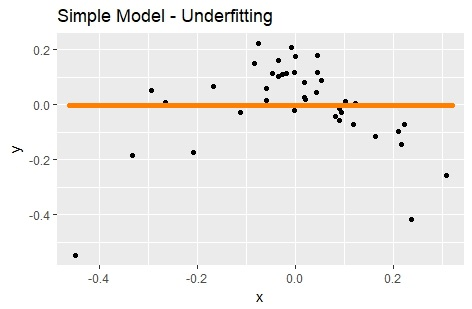
\includegraphics[scale=.5]{figs/plt_underfit.jpg}
        }
    \end{minipage}%
    \begin{minipage}{.5\linewidth}
        \centering
        \subfloat[A overfitting model]{
            \label{fig:overfit}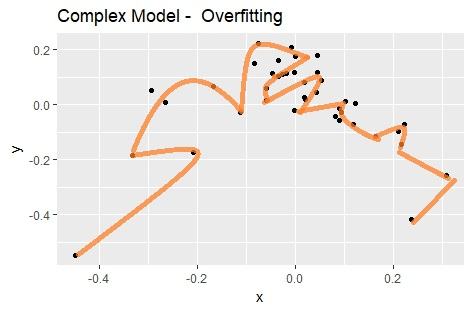
\includegraphics[scale=.5]{figs/plt_overfit.jpg}
        }
    \end{minipage}\par\medskip
    \centering
    \subfloat[The underlying model]{
        \label{main:c}
        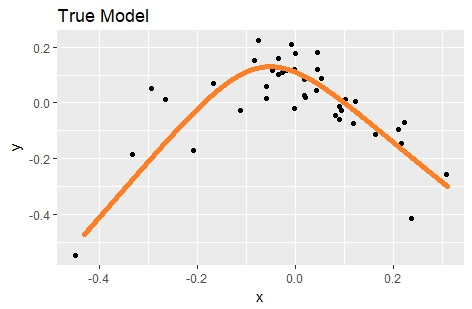
\includegraphics[scale=.5]{figs/plt_true.png}
        }
    \label{fig:main}
    \caption{Plots underfitting, overfitting, and underlying model
             from \cite{the-bias-variance-tradeoff}}
\end{figure}


\begin{figure}[!ht]
    \centering
    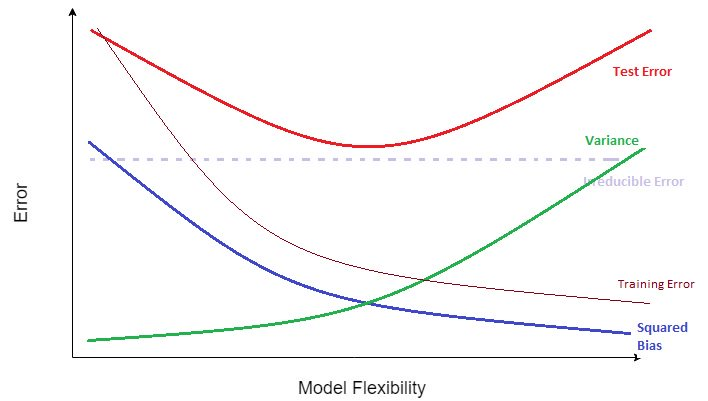
\includegraphics[width=0.8\textwidth]{figs/bias-var-trade.jpg}
    \caption{
        Plot the sq. bias, variance, training error, and test error
        from \cite{the-bias-variance-tradeoff}
    }
    \label{fig:bias-vars-tradeoff}
\end{figure}

% ---------------------------------------------------------------------
\pagebreak

\bibliographystyle{unsrt}
\bibliography{ref}
\pagebreak
\appendix
\section{Appendix}
\subsection*{Question 4a: Simple implemention for adding up digits}
\lstinputlisting{../rnn_add_digits.py}
\subsection*{Question 4b: Tensorflow implemention of XOR neural networks}
\lstinputlisting{../xor_fun.py}

\end{document}
